\subsubsection{\stid{1.16} SICM}
\paragraph{Overview} \leavevmode \\
The goal of this project is to create a universal interface for discovering, managing and sharing within complex memory hierarchies. The result will be a memory API and a software library which implements it. These will allow operating system, runtime and application developers and vendors to access emerging memory technologies. The impact of the project will be immediate and potentially wide reaching, as developers in all areas are struggling to add support for the new memory technologies, each of which offers their own programming interface. 

\paragraph{Key  Challenges} \leavevmode \\
The challenge SICM addresses is how to program the deluge of existing and emerging complex memory technologies on HPC systems. This includes the High Bandwidth Memory (HBM), MCDRAM (on Intel Knights Landing), NV-DIMM, PCI-E NVM, SATA NVM, PCM, memristor, and 3Dxpoint. Also, near node technologies, such as disaggregated memory or network attached memories, have been proposed in exascale memory designs. Current practice depends on ad hoc solutions rather than a uniform API that provides the needed specificity and portability. This approach is already insufficient and future memory technologies will only exacerbate the problem by adding additional proprietary APIs. 

\paragraph{Solution Strategy} \leavevmode \\
The SICM solution is to provide a unified two-tier node-level complex memory API. The target for the low-level interface are system and runtime developers, as well as expert application developers that prefer full control of what memory types the application is using. 
The SICM high-level interface employs application profiling and analysis to direct data management across complex memory hierarchy. The earlier approach is based on an offline profiling approach called MemBrain. The team extended the SICM high-level interface with facilities to profile, analyze, and migrate application data within the same program run. This online approach, Figure~\ref{fig:sicm-online}, reduces user burden and achieves similar performance to the earlier offline approach after a short initial startup period.
The low-level interface is primarily an engineering and implementation project. The solution it provides is urgently needed by the HPC community; as developers work independently to support these novel memory technologies, time and effort is wasted on redundant solutions and overlapping implementations. Adoption of the software is focused on absorption into existing open source projects such as hwloc, KOKKOS, Umpire, CLANG/LLVM, OpenMP, and Jemalloc.
Additionally, SICM is developing Metall, a persistent memory allocator designed to provide developers with an API to allocate custom C++ data structures in both block-storage and byte- addressable persistent memories (e.g., NVMe and Intel Optane DC Persistent Memory) beyond a single process lifetime. Metall relies on a file-backed mmap mechanism to map a file in a filesystem into the virtual memory of an application, allowing the application to access the mapped region as if it were regular memory which can be larger than the physical main-memory of the system.

\paragraph{Recent Progress} \leavevmode 
\begin{itemize}
	\item  Low-Level Interface: Finished refactor of low-level interface supporting memory arenas on different memory types. Added support for Umpire, OpenMP and KOKKOS. Investigating features need to fully support these runtimes, currently KOKKOS and the Nalu-wind ECP application. SICM now supports Intel Optane memory, the first NVM memory that can be used as an extension of traditional DRAM memory.
	Pull requests have been developed for OpenMP/CLANG/LLVM, KOKKOS and Umpire. the patches to Clang/LLVM/OpenMP turn OpenMP memory spaces in OpenMP 5.x into SICM library calls in the LLVM/OpenMP runtime. The same codepath that supports memkind library was refactored to support multiple custom memory allocators – more general than just SICM support.
	SICM currently supports ``pragma openmp allocate'' with  memory types: omp\_ (default, large\_cap, const, high\_bw, low\_lat ) \_mem\_spaces and supports KNL, Optane, testing on Sierra/Summit.  SICM continues to target the early access systems for Frontier and Aurora.
	%Recently, SICM has been ported, compiled and tested on the early access system for Frontier and Aurora.
	\item High-Level API: SICM has employed application profiling and analysis to direct data management across complex memory hierarchy, the team extended the SICM high-level interface with application-directed data tiering based on the MemBrain approach which is more effective than an unguided first touch policy.  The impact of using different data features to steer hot program data into capacity-constrained device tiers was modeled.
	\item  High-Level Graph Interface: For the Metall high-level interface focusing on graph applications, work has used miniVite, and ECP graph proxy application. miniVit has been modified to store and reuse graph data using Metall.  Graph generation has been a bottleneck in this application. Metall can use mmap and UMap (user-level mmap library in Argo PowerSteering project) underneath to enhance its performance and capability.
\end{itemize}

\paragraph{Next Steps} \leavevmode 
\begin{itemize}
	\item  Low-Level Interface: Focus on performance of support for runtimes and adding feature requested to support Umpire, OpenMP KOKKOS, and MPI and address the slow move pages implementation in the Linux kernel. Initial efforts to accelerate move pages have not been sucessful and progress has been hampered by current work environment. The Linux kernel modifications for page migration are in collaboration with ECP project Argo 2.3.5.05 and RIKEN research center in Japan. Start collaborating with applications to enable use of heterogenous memory on ECP target platforms. Additionally, the team needs to reconnect with the hwloc team on memory topology discovery.
	\item For the high-level interface analysis work, the team will adapt their approach and toolset to remove dependence on source code analysis and recompilation of the target application. The goal is to enable guided data management for arbitrary processes, even if source code is not available. The new tools will also integrate with the Linux memory manager in order to direct data management for multiple processes running on the same platform simultaneously.
	\item Metall will continue its collaboration with the ExaGraph team to integrate Metall into an ExaGraph application or benchmark to enable persistent and external-memory data structure support.   
\end{itemize}

\begin{figure}[htb]
	\centering
	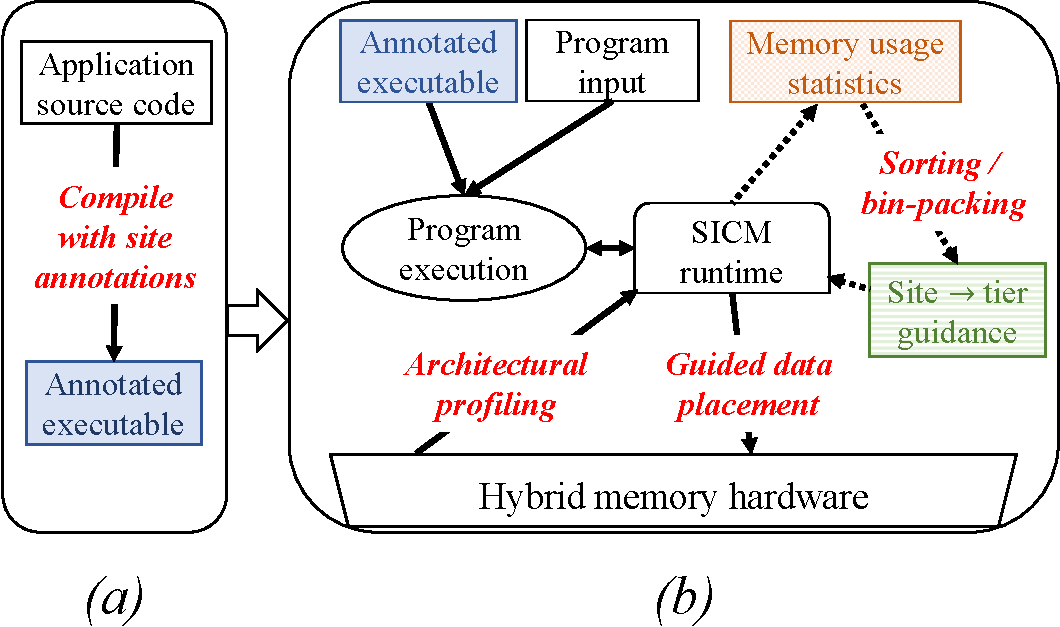
\includegraphics[width=0.7\textwidth]{projects/2.3.1-PMR/2.3.1.16-SICM/sicm-online-diagram.pdf}
	\caption{
		Data tiering with online application guidance. (a) Users first compile the application with a custom pass to insert annotations at each allocation call site, (b) Program execution proceeds inside the SICM runtime layer, which automatically profiles memory usage behavior, converts it into tier recommendations for each allocation site, and enforces these recommendations during program execution. In (b), interactions and operations drawn with dashed lines only occur at regular, timer-based intervals, while the solid lines correspond to activities that can occur throughout the program execution~\cite{olson2021online}.
		\label{fig:sicm-online}
	}
\end{figure}